\chapter{Equilibrio dei corpi solidi}

Nel capitolo precedente abbiamo introdotto le forze e le loro operazioni. Ora ci chiediamo: sotto quali condizioni un corpo, soggetto a più forze, resta fermo? La risposta dipende da come schematizziamo il corpo. Cominciamo dal caso più semplice, il punto materiale; passeremo poi al corpo rigido, in cui una forza può produrre anche una rotazione.

\section{L'equilibrio di un punto materiale}

\begin{definizione}
Un corpo è in \textbf{equilibrio} quando la sua posizione non cambia al passare del tempo.
\end{definizione}

Una biglia appoggiata sul tavolo, un'automobile parcheggiata, un quadro appeso alla parete sono esempi di corpi in equilibrio.

Chiamiamo \textbf{punto materiale} un corpo le cui dimensioni sono trascurabili rispetto al contesto in cui si trova: una biglia rispetto alla stanza, una nave rispetto all'oceano. Un punto materiale non ha forma né dimensioni, ma ha una massa, quindi è soggetto alla forza-peso.

\subsection{La condizione di equilibrio}
Sappiamo che una forza può cambiare lo stato di moto di un corpo. Se un punto materiale è fermo e la risultante delle forze applicate è nulla, esso resta fermo:

\begin{definizione}
Un punto materiale è in equilibrio se e solo se la \textbf{risultante di tutte le forze} applicate è nulla:
\[
\colorboxed{ocre}{\; \vec{R} = \vec{F}_1 + \vec{F}_2 + \vec{F}_3 + \dots = \vec{0} \;}
\]
\end{definizione}

Per esempio, se su una palla da biliardo agiscono due forze uguali e opposte di modulo $\SI{20}{\newton}$, la risultante è nulla e la palla non si muove.

\subsection{Vincoli e reazioni vincolari}
Consideriamo la biglia ferma sul tavolo. Su di essa agisce la forza-peso $\vec{P}$, diretta verso il basso: se questa fosse l'unica forza, la biglia cadrebbe. Deve quindi agire un'altra forza, uguale e opposta, esercitata dal tavolo.

\begin{definizione}
Un \textbf{vincolo} è un corpo che, esercitando una forza, impedisce a un altro corpo di compiere certi movimenti. La forza esercitata da un vincolo si chiama \textbf{reazione vincolare} $\vec{R}_v$.
\end{definizione}

Il tavolo impedisce alla biglia di muoversi verso il basso: la reazione vincolare $\vec{R}_v$ è diretta verso l'alto e la biglia è in equilibrio:
\[
\vec{R}_v + \vec{P} = \vec{0} \qquad \Longrightarrow \qquad \vec{R}_v = -\vec{P}.
\]
Altri esempi di vincolo: i binari, che costringono il treno a muoversi in una sola direzione; il gancio di una gru, che sostiene un carico.

\begin{figure}[h!]
\centering
\begin{tikzpicture}[scale=1,>=stealth]
\draw[thick] (-1.6,0) -- (1.6,0);
\foreach \x in {-1.2,-0.6,0,0.6,1.2}{\draw (\x,0) -- (\x-0.25,-0.35);}
\shade[ball color=orange!60] (0,0.45) circle (0.45);
\draw[->,very thick,ocre] (0,0.45) -- (0,-1.1) node[right,black]{$\vec{P}$};
\draw[->,very thick,blue!60!black] (0,0.45) -- (0,2) node[right,black]{$\vec{R}_v$};
\end{tikzpicture}
\caption{La biglia sul tavolo è in equilibrio: la reazione vincolare $\vec{R}_v$ bilancia il peso $\vec{P}$.}
\label{fig:biglia}
\end{figure}

\subsection{La forza equilibrante}
Quando un punto materiale \emph{non} è in equilibrio, per equilibrarlo basta aggiungere una forza uguale e opposta alla risultante delle forze già applicate: questa si chiama \textbf{forza equilibrante} $\vec{F}_e$:
\[
\vec{F}_e = -\vec{R}.
\]
Per esempio, un carico di mattoni di peso $\SI{2000}{\newton}$ tenuto sospeso da una gru è in equilibrio grazie alla \textbf{tensione} $\vec{T}$ del cavo, che è la forza equilibrante: ha modulo $\SI{2000}{\newton}$ ed è diretta verso l'alto.

\begin{testexample}[\thetcbcounter \, Lampada appesa a due fili]
Una lampada di peso $\SI{30}{\newton}$ è appesa al soffitto tramite due fili verticali che sostengono metà del peso ciascuno. Qual è la tensione di ogni filo? Poiché la lampada è in equilibrio, la somma delle due tensioni (verso l'alto) deve bilanciare il peso (verso il basso): $T_1 + T_2 = \SI{30}{\newton}$. Essendo i fili uguali, $T_1 = T_2 = \SI{15}{\newton}$.
\end{testexample}

\subsection{Esercizi}

\begin{esercizio}
Su un anello agiscono tre forze complanari. Due valgono $\SI{8}{\newton}$ verso Est e $\SI{8}{\newton}$ verso Ovest. Quanto deve valere la terza forza perché l'anello sia in equilibrio?\\
\risp{$\SI{0}{\newton}\ \text{(nulla): le prime due si bilanciano già)}$}
\end{esercizio}

\begin{esercizio}
Un lampadario di peso $\SI{45}{\newton}$ è sostenuto da una catena verticale. Quanto vale la tensione della catena? Come si chiama, rispetto al lampadario, questa forza?\\
\risp{$T = \SI{45}{\newton}\ ;\ \text{forza equilibrante (reazione vincolare del gancio)}$}
\end{esercizio}

\begin{esercizio}
Su un punto materiale agiscono due forze perpendicolari, di moduli $\SI{6}{\newton}$ e $\SI{8}{\newton}$. Quale forza equilibrante bisogna aggiungere per metterlo in equilibrio? (indica modulo e direzione).\\
\risp{$\SI{10}{\newton}\text{, opposta alla risultante delle due forze}$}
\end{esercizio}


\section{L'equilibrio e l'attrito}

\subsection{Un oggetto su un piano inclinato}
Consideriamo un blocco appoggiato su un piano inclinato \textbf{liscio} (senza attrito). Su di esso agiscono la forza-peso $\vec{P}$, verticale verso il basso, e la reazione vincolare $\vec{R}_v$, perpendicolare al piano. Scomponiamo il peso nei vettori componenti $\vec{P}_\parallel$ (parallelo al piano) e $\vec{P}_\perp$ (perpendicolare al piano), come abbiamo fatto nel paragrafo~\ref{sec:scomposizione}.

La reazione vincolare bilancia esattamente $\vec{P}_\perp$: $\vec{R}_v = -\vec{P}_\perp$. Ma la componente $\vec{P}_\parallel$ resta \textbf{non bilanciata}: il blocco scivola verso il basso.

\begin{remark}
Un oggetto non può stare in equilibrio su un piano inclinato liscio senza una forza esterna che ne bilanci la componente $\vec{P}_\parallel$.
\end{remark}

Indicando con $l$ la lunghezza del piano e con $h$ la sua altezza, per considerazioni geometriche si ha:
\[
\colorboxed{ocre}{\; P_\parallel = P\,\frac{h}{l} \;}
\]
che è equivalente a $P_\parallel = P\sin\alpha$, dove $\alpha$ è l'angolo di inclinazione.

\begin{testexample}[\thetcbcounter \, Slitta su un piano inclinato]
Una slitta di peso $\SI{100}{\newton}$ è su un piano inclinato lungo $\SI{2,6}{\meter}$ e alto $\SI{1,3}{\meter}$. La componente del peso parallela al piano vale:
\[
P_\parallel = P\,\frac{h}{l} = \SI{100}{\newton}\times\frac{\SI{1,3}{\meter}}{\SI{2,6}{\meter}} = \SI{50}{\newton}.
\]
Per tenere ferma la slitta serve una forza parallela al piano, diretta verso l'alto, di $\SI{50}{\newton}$.
\end{testexample}

\subsection{Piano inclinato con attrito}
Se il piano non è liscio, entra in gioco la forza di attrito statico $\vec{F}_{as}$, parallela al piano e diretta verso l'alto (si oppone alla tendenza a scivolare). Il blocco è in equilibrio se l'attrito statico riesce a bilanciare $\vec{P}_\parallel$:
\[
F_{as} = P_\parallel .
\]
Ma l'attrito statico non può superare il valore massimo $k_s\,F_p$, dove la forza premente è $F_p = P_\perp$. Dunque il blocco resta fermo finché:
\[
P_\parallel \le k_s\,P_\perp .
\]

\begin{figure}[h!]
\centering
\begin{tikzpicture}[scale=1,>=stealth]
\def\ang{25}
\draw[thick] (0,0) -- (6,0) -- (6,{6*tan(\ang)}) -- cycle;
\draw (1,0) arc (0:\ang:1); \node at (1.45,0.22){\small $\alpha$};
\begin{scope}[shift={(3.3,{3.3*tan(\ang)})},rotate=\ang]
\fill[gray!25] (-0.6,0) rectangle (0.6,0.75);
\draw (-0.6,0) rectangle (0.6,0.75);
\end{scope}
\coordinate (C) at (3.3,{3.3*tan(\ang)+0.37});
\draw[->,very thick,ocre] (C) -- ++(0,-2) node[right,black]{$\vec{P}$};
\draw[->,thick,blue!60!black] (C) -- ++({90+\ang}:1.3) node[above,black]{$\vec{R}_v$};
\draw[->,thick,red!70!black] (C) -- ++({\ang}:1.5) node[above right,black]{$\vec{F}_{as}$};
\end{tikzpicture}
\caption{Blocco fermo su un piano inclinato scabro: la reazione vincolare bilancia $\vec{P}_\perp$, l'attrito statico bilancia $\vec{P}_\parallel$.}
\label{fig:incl-attrito}
\end{figure}

\subsection{L'angolo limite}
Aumentiamo l'inclinazione $\alpha$: la componente $P_\parallel$ cresce, mentre $P_\perp$ (e quindi il massimo dell'attrito) diminuisce. Esiste un angolo $\alpha_0$, detto \textbf{angolo limite}, oltre il quale il blocco scivola comunque. Si può dimostrare che:
\[
\colorboxed{ocre}{\; \tan\alpha_0 = k_s \;}
\]
Notevole: l'angolo limite \textbf{non dipende dalla massa} dell'oggetto, ma solo dal coefficiente di attrito statico. Misurare l'angolo limite di un piano inclinato è quindi un modo per determinare $k_s$.

\begin{testexample}[\thetcbcounter \, Cassa su un piano inclinato]
Una cassa di massa $\SI{5,0}{\kilo\gram}$ è su un piano inclinato di $20^\circ$; il coefficiente di attrito statico è $k_s = 0,50$. La cassa è in equilibrio?

Peso: $P = mg = \SI{49}{\newton}$. Componenti (con $\sin 20^\circ \approx 0,34$, $\cos 20^\circ \approx 0,94$):
\[
P_\parallel \approx \SI{49}{\newton}\times 0,34 \approx \SI{17}{\newton}, \qquad P_\perp \approx \SI{49}{\newton}\times 0,94 \approx \SI{46}{\newton}.
\]
Massimo attrito statico: $k_s\,P_\perp = 0,50 \times \SI{46}{\newton} = \SI{23}{\newton}$. Poiché $P_\parallel = \SI{17}{\newton} < \SI{23}{\newton}$, la cassa \textbf{resta ferma}. (Equivalentemente: $\tan 20^\circ \approx 0,36 < k_s = 0,50$, quindi $\alpha < \alpha_0$.)
\end{testexample}

\subsection{Esercizi}

\begin{esercizio}
Un piano inclinato è lungo $\SI{3,0}{\meter}$ e alto $\SI{1,5}{\meter}$. Un carrello di peso $\SI{80}{\newton}$ vi è appoggiato. Se il piano è liscio, quale forza parallela al piano serve per tenerlo fermo?\\
\risp{$F = \SI{40}{\newton}$}
\end{esercizio}

\begin{esercizio}
Il coefficiente di attrito statico tra un blocco e un piano inclinato vale $k_s = 0,70$. Qual è l'angolo limite? Un blocco più pesante avrebbe un angolo limite diverso?\\
\risp{$\alpha_0 = \arctan 0,70 \approx 35^\circ\ ;\ \text{no, non dipende dalla massa}$}
\end{esercizio}

\begin{esercizio}
Una cassa è ferma su un piano inclinato di $18^\circ$. Misurando l'angolo limite si trova $\alpha_0 = 22^\circ$. La cassa è in equilibrio? Quanto vale, circa, il coefficiente di attrito statico?\\
\risp{$\text{sì}\ (18^\circ < 22^\circ)\ ;\quad k_s = \tan 22^\circ \approx 0,40$}
\end{esercizio}


\section{L'equilibrio di un corpo rigido}

Il modello del punto materiale permette di studiare oggetti che possono solo \emph{traslare}. Per studiare oggetti che possono anche \emph{ruotare} serve un modello più ricco.

\begin{definizione}
Un \textbf{corpo rigido} è un oggetto dotato di forma e dimensioni, che non subisce deformazioni anche se soggetto a forze.
\end{definizione}

\subsection{Il braccio e il momento di una forza}
Consideriamo una chiave inglese usata per svitare un bullone. La chiave può ruotare attorno al bullone; osserviamo come cambia la facilità di rotazione al variare della forza applicata:
\begin{itemize}
\item una forza più \textbf{intensa} fa ruotare più facilmente il bullone;
\item una forza applicata in un punto più \textbf{lontano} dal bullone lo fa ruotare più facilmente di una forza uguale applicata vicino;
\item una forza diretta \textbf{verso} il centro di rotazione non lo fa ruotare affatto.
\end{itemize}
L'effetto rotatorio di una forza dipende quindi dalla sua intensità, dal suo punto di applicazione e dalla sua direzione. Queste tre informazioni si riassumono in un'unica grandezza. Chiamiamo \textbf{braccio} della forza $b$ la distanza tra il centro di rotazione $O$ e la retta d'azione della forza (figura~\ref{fig:momento}).

\begin{figure}[h!]
\centering
\begin{tikzpicture}[scale=1,>=stealth]
\fill (0,0) circle (1.5pt) node[below left]{$O$};
\draw[thick] (0,0) -- (3.6,0);
\fill[gray!30] (3.2,-0.18) rectangle (3.9,0.18);
\draw[->,very thick,ocre] (3.55,0) -- (3.55,-1.6) node[right,black]{$\vec{F}$};
\draw[dashed,gray] (3.55,0.4) -- (3.55,-1.8);
\draw[<->] (0,0.45) -- (3.55,0.45) node[midway,above]{$b$};
\draw[dotted] (0,0) -- (0,0.55);
\draw[dotted] (3.55,0) -- (3.55,0.55);
\end{tikzpicture}
\caption{Il braccio $b$ di una forza è la distanza tra il centro di rotazione $O$ e la retta d'azione della forza.}
\label{fig:momento}
\end{figure}

\begin{definizione}
Il \textbf{momento} di una forza $\vec{F}$ rispetto a un punto $O$ è il prodotto dell'intensità della forza per il suo braccio:
\[
\colorboxed{ocre}{\; M = F\cdot b \;}
\]
Nel Sistema Internazionale si misura in \textbf{newton per metro} ($\si{\newton\meter}$).
\end{definizione}

Per \textbf{convenzione}, il momento è \textbf{positivo} se la forza tende a far ruotare il corpo in senso antiorario, \textbf{negativo} se in senso orario. Se la retta d'azione passa per $O$, il braccio è nullo e il momento è nullo: la forza non produce rotazione.

\begin{testexample}[\thetcbcounter \, Momento su una chiave]
Su una chiave inglese si applica una forza di $\SI{100}{\newton}$ perpendicolare alla chiave, a $\SI{20}{\centi\meter}$ dal bullone. Il momento della forza rispetto al bullone è:
\[
M = F\cdot b = \SI{100}{\newton}\times\SI{0,20}{\meter} = \SI{20}{\newton\meter}.
\]
\end{testexample}

\subsection{Le condizioni per l'equilibrio di un corpo rigido}
Un corpo rigido può traslare (se la risultante delle forze non è nulla) e ruotare (se la somma dei momenti non è nulla). Perché sia in equilibrio devono valere \textbf{entrambe} le condizioni:

\begin{definizione}
Un corpo rigido è in equilibrio se e solo se:
\begin{enumerate}
\item la risultante di tutte le forze applicate è nulla \quad ($\vec{R} = \vec{F}_1 + \vec{F}_2 + \dots = \vec{0}$) \quad — \emph{equilibrio alla traslazione};
\item la somma dei momenti di tutte le forze, calcolati rispetto a uno stesso punto, è nulla \quad ($M_1 + M_2 + \dots = 0$) \quad — \emph{equilibrio alla rotazione}.
\end{enumerate}
\end{definizione}

\begin{figure}[h!]
\centering
\begin{tikzpicture}[scale=1,>=stealth]
\draw[thick] (-2,0) -- (1.5,0);
\fill[gray!40] (-0.25,-0.5) -- (0.25,-0.5) -- (0,0) -- cycle;
\fill (0,0) circle (1.2pt) node[above=2pt]{$O$};
\fill (-2,0) circle (1.2pt);
\fill (1.5,0) circle (1.2pt);
\draw[->,very thick,ocre] (-2,0) -- (-2,-1.4) node[below,black]{$\vec{F}_1$};
\draw[->,very thick,ocre] (1.5,0) -- (1.5,-1.1) node[below,black]{$\vec{F}_2$};
\draw[<->] (-2,0.4) -- (0,0.4) node[midway,above]{$b_1$};
\draw[<->] (0,0.4) -- (1.5,0.4) node[midway,above]{$b_2$};
\end{tikzpicture}
\caption{Asta appoggiata su un fulcro $O$: è in equilibrio alla rotazione se $F_1 b_1 = F_2 b_2$ (i due momenti sono uguali e opposti).}
\label{fig:asta}
\end{figure}

\begin{testexample}[\thetcbcounter \, Altalena in equilibrio]
Su un'altalena, il cui fulcro è al centro, un bambino di peso $\SI{300}{\newton}$ si siede a $\SI{2,0}{\meter}$ dal fulcro. A quale distanza deve sedersi, dall'altra parte, un bambino di peso $\SI{400}{\newton}$ perché l'altalena sia in equilibrio?

I due momenti devono essere uguali e opposti: $P_1\,b_1 = P_2\,b_2$, quindi
\[
b_2 = \frac{P_1\,b_1}{P_2} = \frac{\SI{300}{\newton}\times\SI{2,0}{\meter}}{\SI{400}{\newton}} = \SI{1,5}{\meter}.
\]
Il bambino più pesante deve sedersi più vicino al fulcro.
\end{testexample}

\subsection{Esercizi}

\begin{esercizio}
Una forza di $\SI{30}{\newton}$ è applicata perpendicolarmente a una porta, a $\SI{15}{\centi\meter}$ dai cardini. Quanto vale il momento della forza rispetto ai cardini? Perché le maniglie si mettono lontano dai cardini?\\
\risp{$M = \SI{4,5}{\newton\meter}\ ;\ \text{per avere un braccio grande e quindi un momento maggiore}$}
\end{esercizio}

\begin{esercizio}
Un'asta è appoggiata su un fulcro. A sinistra, a $\SI{80}{\centi\meter}$ dal fulcro, agisce verso il basso una forza di $\SI{250}{\newton}$. A destra, a $\SI{50}{\centi\meter}$ dal fulcro, quale forza verso il basso mantiene l'asta in equilibrio?\\
\risp{$F = \SI{400}{\newton}$}
\end{esercizio}

\begin{esercizio}
Una chiave dinamometrica è regolata per un momento massimo di $\SI{40}{\newton\meter}$: oltre questo valore ``slitta'' e non stringe di più. Se la chiave è lunga $\SI{40}{\centi\meter}$ e si applica la forza all'estremità, qual è la massima forza applicabile?\\
\risp{$F = \SI{100}{\newton}$}
\end{esercizio}


\section{Le coppie di forze}

\begin{definizione}
Due forze parallele, di uguale intensità e verso opposto, applicate in punti diversi di uno stesso corpo rigido, formano una \textbf{coppia di forze}.
\end{definizione}

La risultante di una coppia è \textbf{nulla}, quindi il corpo non trasla; tuttavia il corpo \textbf{ruota}, perché ciascuna delle due forze produce una rotazione nello stesso senso. È quello che facciamo quando giriamo un volante con le due mani, o svitiamo un tappo con due dita.

Si chiama \textbf{braccio della coppia} $b$ la distanza tra le rette d'azione delle due forze. Il \textbf{momento della coppia} è:
\[
\colorboxed{ocre}{\; M = F\cdot b \;}
\]
Una proprietà importante: il momento di una coppia è lo stesso rispetto a qualunque punto si scelga (non dipende dal polo).

\begin{figure}[h!]
\centering
\begin{tikzpicture}[scale=1,>=stealth]
\draw[thick,gray!50] (-2.5,0.6) -- (2.5,-0.6);
\draw[->,very thick,ocre] (-2,0.48) -- (-2,1.7) node[above,black]{$\vec{F}$};
\draw[->,very thick,ocre] (2,-0.48) -- (2,-1.7) node[below,black]{$-\vec{F}$};
\draw[dashed,gray] (-2,0.48) -- (-2,-1.5);
\draw[dashed,gray] (2,-0.48) -- (2,1.5);
\draw[<->] (-2,-1.0) -- (2,-1.0) node[midway,fill=white]{$b$};
\end{tikzpicture}
\caption{Una coppia di forze: risultante nulla, ma momento $M = F\,b$ non nullo. Il corpo ruota.}
\label{fig:coppia}
\end{figure}

Come per il momento di una singola forza, si assume positivo il momento della coppia che produce una rotazione antioraria, negativo quello che produce una rotazione oraria.

\begin{testexample}[\thetcbcounter \, Il volante]
Un automobilista gira il volante applicando alle due estremità di un diametro (lungo $\SI{36}{\centi\meter}$) due forze uguali e opposte di $\SI{20}{\newton}$: si tratta di una coppia. Il suo momento è:
\[
M = F\cdot b = \SI{20}{\newton}\times\SI{0,36}{\meter} \approx \SI{7,2}{\newton\meter}.
\]
\end{testexample}

\subsection{Esercizi}

\begin{esercizio}
Su un righello agiscono due forze di $\SI{5}{\newton}$, parallele e di verso opposto, le cui rette d'azione distano $\SI{20}{\centi\meter}$. Qual è la risultante? Qual è il momento della coppia? Il righello ruota?\\
\risp{$\vec{R} = \vec{0}\ ;\quad M = \SI{1}{\newton\meter}\ ;\quad \text{sì, ruota}$}
\end{esercizio}

\begin{esercizio}
Per svitare un tappo si applicano con due dita due forze di $\SI{8}{\newton}$ ai due lati del tappo, di diametro $\SI{4,0}{\centi\meter}$. Quanto vale il momento della coppia?\\
\risp{$M = \SI{0,32}{\newton\meter}$}
\end{esercizio}

\begin{esercizio}
Spiega la differenza tra una coppia di forze e due forze qualsiasi uguali e opposte applicate nello stesso punto.\\
\risp{$\text{stesso punto} \Rightarrow \text{risultante e momento nulli, equilibrio; punti diversi} \Rightarrow \text{coppia, il corpo ruota}$}
\end{esercizio}


\section{Le macchine semplici e le leve}

\begin{definizione}
Una \textbf{macchina semplice} è un dispositivo che permette di equilibrare o vincere una forza (detta \textbf{forza resistente} $\vec{F}_r$) applicandone un'altra di intensità o direzione diversa (detta \textbf{forza motrice} $\vec{F}_m$).
\end{definizione}

Per valutare la convenienza di una macchina si usa il \textbf{guadagno}:
\[
\colorboxed{ocre}{\; G = \frac{F_r}{F_m} \;}
\]
È un numero puro (senza unità di misura). Una macchina è:
\begin{itemize}
\item \textbf{vantaggiosa} se $G > 1$ (la forza motrice è minore della resistente);
\item \textbf{svantaggiosa} se $G < 1$;
\item \textbf{indifferente} se $G = 1$.
\end{itemize}

\subsection{Le leve}
La macchina semplice più comune è la \textbf{leva}: un corpo rigido di forma allungata che può ruotare attorno a un punto fisso, il \textbf{fulcro}. Chiamiamo $b_m$ e $b_r$ i \textbf{bracci} della forza motrice e della forza resistente rispetto al fulcro. Perché la leva sia in equilibrio, i momenti delle due forze devono essere uguali e opposti:
\[
\colorboxed{ocre}{\; F_m\,b_m = F_r\,b_r \;}
\]
Da qui si ricava che il guadagno di una leva dipende solo dai bracci:
\[
G = \frac{F_r}{F_m} = \frac{b_m}{b_r}.
\]
Una leva è vantaggiosa quando il braccio della forza motrice è maggiore di quello della forza resistente.

\subsection{I tre generi di leva}
A seconda della posizione del fulcro rispetto alle due forze, si distinguono tre generi di leva.

\paragraph{Leva di primo genere.} Il fulcro è \emph{tra} le due forze (figura~\ref{fig:leva1}). Può essere vantaggiosa, svantaggiosa o indifferente, a seconda dei bracci. Esempi: l'altalena, le forbici, la tenaglia, la bilancia a bracci uguali (leva indifferente).

\begin{figure}[h!]
\centering
\begin{tikzpicture}[scale=1,>=stealth]
\draw[thick] (-2.3,0) -- (1.6,0);
\fill (-2.3,0) circle (1.1pt);  \fill (1.6,0) circle (1.1pt);
\fill[gray!45] (-0.28,-0.5) -- (0.28,-0.5) -- (0,0) -- cycle;
\node[below=6pt] at (0,-0.5) {\small fulcro};
\draw[<->] (-2.3,0.5) -- (0,0.5) node[midway,above]{\small $b_m$};
\draw[<->] (0,0.5) -- (1.6,0.5) node[midway,above]{\small $b_r$};
\draw[->,very thick,red!70!black] (-2.3,0) -- (-2.3,-1.2) node[below,black]{$\vec{F}_m$};
\draw[->,very thick,ocre] (1.6,0) -- (1.6,-1.5) node[below,black]{$\vec{F}_r$};
\end{tikzpicture}
\caption{Leva di primo genere: il fulcro è tra la forza motrice e la forza resistente.}
\label{fig:leva1}
\end{figure}

\paragraph{Leva di secondo genere.} La forza resistente è \emph{tra} il fulcro e la forza motrice (figura~\ref{fig:leva2}). È \textbf{sempre vantaggiosa}, perché $b_m > b_r$. Esempi: la carriola, lo schiaccianoci, il remo (in parte).

\begin{figure}[h!]
\centering
\begin{tikzpicture}[scale=1,>=stealth]
\draw[thick] (0,0) -- (3.8,0);
\fill (0,0) circle (1.1pt);  \fill (3.8,0) circle (1.1pt);
\fill[gray!45] (-0.28,-0.5) -- (0.28,-0.5) -- (0,0) -- cycle;
\node[below=6pt] at (0,-0.5) {\small fulcro};
\draw[<->] (0,0.5) -- (2,0.5) node[midway,above]{\small $b_r$};
\draw[<->] (0,1.6) -- (3.8,1.6) node[midway,above]{\small $b_m$};
\draw[->,very thick,ocre] (2,0) -- (2,-1.5) node[below,black]{$\vec{F}_r$};
\draw[->,very thick,red!70!black] (3.8,0) -- (3.8,1.4) node[right,black]{$\vec{F}_m$};
\end{tikzpicture}
\caption{Leva di secondo genere: la forza resistente è tra il fulcro e la forza motrice. Sempre vantaggiosa ($b_m > b_r$).}
\label{fig:leva2}
\end{figure}

\paragraph{Leva di terzo genere.} La forza motrice è \emph{tra} il fulcro e la forza resistente (figura~\ref{fig:leva3}). È \textbf{sempre svantaggiosa}, perché $b_m < b_r$. In compenso, permette al punto di applicazione della resistenza di spostarsi molto e velocemente. Esempi: l'avambraccio (il bicipite è la forza motrice), le pinzette, la canna da pesca.

\begin{figure}[h!]
\centering
\begin{tikzpicture}[scale=1,>=stealth]
\draw[thick] (0,0) -- (3.8,0);
\fill (0,0) circle (1.1pt);  \fill (3.8,0) circle (1.1pt);
\fill[gray!45] (-0.28,-0.5) -- (0.28,-0.5) -- (0,0) -- cycle;
\node[below=6pt] at (0,-0.5) {\small fulcro};
\draw[<->] (0,0.5) -- (1.3,0.5) node[midway,above]{\small $b_m$};
\draw[<->] (0,2.2) -- (3.8,2.2) node[midway,above]{\small $b_r$};
\draw[->,very thick,red!70!black] (1.3,0) -- (1.3,1.5) node[above,black]{$\vec{F}_m$};
\draw[->,very thick,ocre] (3.8,0) -- (3.8,-1.5) node[below,black]{$\vec{F}_r$};
\end{tikzpicture}
\caption{Leva di terzo genere: la forza motrice è tra il fulcro e la forza resistente. Sempre svantaggiosa ($b_m < b_r$).}
\label{fig:leva3}
\end{figure}

\begin{testexample}[\thetcbcounter \, Sollevare un masso con una leva]
Vogliamo sollevare un masso di peso $F_r = \SI{1000}{\newton}$ facendo leva con una sbarra. Il fulcro (una pietra d'appoggio) è a $b_r = \SI{0,20}{\meter}$ dal masso, e spingiamo l'altro estremo della sbarra a $b_m = \SI{1,0}{\meter}$ dal fulcro. Che forza dobbiamo esercitare?
\[
F_m = \frac{F_r\,b_r}{b_m} = \frac{\SI{1000}{\newton}\times\SI{0,20}{\meter}}{\SI{1,0}{\meter}} = \SI{200}{\newton}.
\]
Il guadagno è $G = b_m/b_r = 5$: la leva è vantaggiosa.
\end{testexample}

\begin{testexample}[\thetcbcounter \, L'avambraccio]
L'avambraccio è una leva di terzo genere: il fulcro è il gomito, la forza motrice è quella del bicipite (applicata a circa $b_m = \SI{4}{\centi\meter}$ dal gomito), la forza resistente è il peso sostenuto dalla mano (a circa $b_r = \SI{35}{\centi\meter}$ dal gomito). Per sostenere un peso di $\SI{50}{\newton}$ il bicipite deve esercitare:
\[
F_m = \frac{F_r\,b_r}{b_m} = \frac{\SI{50}{\newton}\times\SI{35}{\centi\meter}}{\SI{4}{\centi\meter}} \approx \SI{440}{\newton}.
\]
Il guadagno è circa $0,11$: molto svantaggiosa in termini di forza, ma la mano si muove su un arco ampio con piccoli accorciamenti del muscolo.
\end{testexample}

\subsection{Esercizi}

\begin{esercizio}
Per sollevare un peso di $\SI{4500}{\newton}$ si usa una leva con guadagno $G = 6$. Quale forza motrice bisogna applicare?\\
\risp{$F_m = \SI{750}{\newton}$}
\end{esercizio}

\begin{esercizio}
Una leva ha braccio della forza motrice $b_m = \SI{90}{\centi\meter}$ e braccio della forza resistente $b_r = \SI{30}{\centi\meter}$. Qual è il guadagno? La leva è vantaggiosa o svantaggiosa?\\
\risp{$G = 3\ ;\ \text{vantaggiosa}$}
\end{esercizio}

\begin{esercizio}
In una carriola (leva di secondo genere) il carico pesa $\SI{800}{\newton}$ ed è a $\SI{30}{\centi\meter}$ dalla ruota; le stanghe si impugnano a $\SI{1,5}{\meter}$ dalla ruota. Quale forza deve applicare chi la solleva?\\
\risp{$F_m = \SI{160}{\newton}$}
\end{esercizio}

\begin{esercizio}
Uno schiaccianoci è una leva di secondo genere: si applica una forza di $\SI{40}{\newton}$ all'estremità dei manici, a $\SI{12}{\centi\meter}$ dalla cerniera, mentre la noce è a $\SI{3}{\centi\meter}$ dalla cerniera. Con quale forza viene schiacciata la noce?\\
\risp{$F_r = \SI{160}{\newton}$}
\end{esercizio}

\begin{esercizio}
Per ciascuno di questi attrezzi indica il genere di leva: pinzetta da sopracciglia, tenaglia, carriola, remo, altalena.\\
\risp{terzo; primo; secondo; secondo; primo}
\end{esercizio}


\section{Il baricentro e l'equilibrio}

\subsection{Centro di simmetria e baricentro}
Alcuni corpi solidi hanno un \textbf{centro di simmetria}: il cubo, la sfera, il parallelepipedo. I corpi di forma irregolare non ne hanno. Un corpo si dice \textbf{omogeneo} se la sua densità è la stessa in ogni sua parte; il martello, per esempio, non è omogeneo, perché la testa di ferro e il manico di legno hanno densità diverse.

Il peso di un corpo è la somma dei pesi di tutte le sue particelle: è una forza distribuita su tutto il volume. Possiamo però pensare che il peso sia concentrato in un unico punto.

\begin{definizione}
Il \textbf{baricentro} (o centro di gravità) è il punto in cui si può considerare applicata l'intera forza-peso di un corpo.
\end{definizione}

Per un corpo \textbf{omogeneo e regolare}, il baricentro coincide con il centro di simmetria: al centro per una sfera o un cubo, nel punto d'incontro delle diagonali per un rettangolo. Per un corpo irregolare o non omogeneo (come una mazza da baseball, più pesante da un lato) il baricentro è spostato verso la parte più pesante e va cercato per via sperimentale.

\begin{remark}
Il baricentro è un punto \textbf{immaginario}: non deve necessariamente trovarsi dentro il materiale del corpo. Per un anello o un ferro di cavallo, per esempio, il baricentro cade nel vuoto.
\end{remark}

\subsection{Ricerca sperimentale del baricentro}
Per trovare il baricentro di un corpo piatto e irregolare (per esempio un cartoncino ritagliato) si procede così:
\begin{enumerate}
\item si appende il corpo a un chiodo, per un punto $A_1$ del bordo, e lo si lascia oscillare fino a fermarsi. All'equilibrio il baricentro si trova sulla \textbf{verticale} passante per $A_1$: se non lo fosse, peso e reazione del chiodo formerebbero una coppia che farebbe ancora ruotare il corpo;
\item si appende allo stesso chiodo un \textbf{filo a piombo} e si traccia sul corpo la retta verticale $r_1$;
\item si ripete l'operazione appendendo il corpo per un altro punto $A_2$, e si traccia la retta $r_2$.
\end{enumerate}
Il baricentro $B$ è il punto di \textbf{intersezione} delle due rette (figura~\ref{fig:baricentro}). Una terza sospensione serve solo come verifica: la sua verticale passa per lo stesso punto.

\begin{figure}[h!]
\centering
\begin{tikzpicture}[scale=1,>=stealth]
\coordinate (A1) at (0.7,2.1);
\coordinate (A2) at (2.2,0.8);
\coordinate (B) at (1.05,1.0);
% corpo irregolare
\draw[fill=gray!15,thick] (0,0) -- (1.6,-0.3) -- (2.2,0.8) -- (1.8,1.9) -- (0.7,2.1) -- (-0.2,1.2) -- cycle;
% rette tracciate col filo a piombo
\draw[ocre,dashed] (A1) -- ($(A1)!1.75!(B)$) node[pos=1,below]{\small $r_1$};
\draw[blue!55!black,dashed] (A2) -- ($(A2)!1.95!(B)$) node[pos=1,left]{\small $r_2$};
% chiodi
\fill (A1) circle (1.6pt) node[above]{\small $A_1$};
\fill (A2) circle (1.6pt) node[right]{\small $A_2$};
% baricentro
\fill[red] (B) circle (1.8pt) node[above right]{\small $B$};
\end{tikzpicture}
\caption{Ricerca del baricentro: le verticali tracciate col filo a piombo appendendo il corpo per $A_1$ e per $A_2$ si incontrano nel baricentro $B$.}
\label{fig:baricentro}
\end{figure}

\subsection{Equilibrio stabile, instabile e indifferente}
Non tutti gli equilibri si comportano allo stesso modo. Pensiamo a una pallina appoggiata su tre superfici diverse (figura~\ref{fig:stab}) e immaginiamo di spostarla di poco dalla sua posizione:
\begin{itemize}
\item sul \textbf{fondo di una cunetta} la pallina, lasciata libera, torna indietro fino al punto più basso: l'equilibrio è \textbf{stabile};
\item sulla \textbf{sommità di una collinetta} la pallina rotola via e si allontana sempre di più: l'equilibrio è \textbf{instabile};
\item su un \textbf{piano orizzontale} la pallina resta ferma nella nuova posizione: l'equilibrio è \textbf{indifferente}.
\end{itemize}

\begin{figure}[h!]
\centering
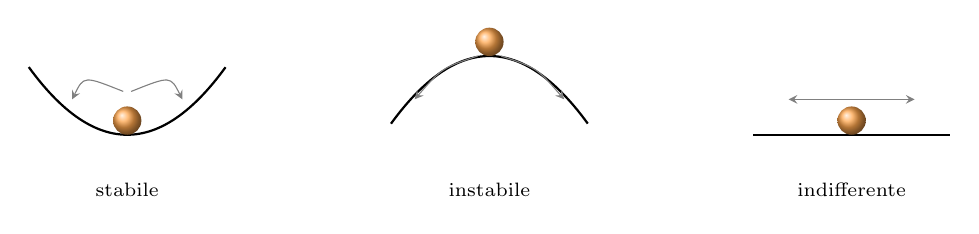
\begin{tikzpicture}[scale=1,>=stealth]
% stabile: pallina nel fondo di una cunetta
\begin{scope}
\draw[thick,domain=-1.25:1.25,samples=60] plot (\x,{0.55*\x*\x});
\shade[ball color=orange!70] (0,0.18) circle (0.18);
\draw[->,gray] (0.05,0.55) .. controls (0.55,0.75) .. (0.7,0.45);
\draw[<-,gray] (-0.7,0.45) .. controls (-0.55,0.75) .. (-0.05,0.55);
\node at (0,-0.7) {\scriptsize stabile};
\end{scope}
% instabile: pallina sulla sommita' di una collinetta
\begin{scope}[xshift=4.6cm]
\draw[thick,domain=-1.25:1.25,samples=60] plot (\x,{1-0.55*\x*\x});
\shade[ball color=orange!70] (0,1.18) circle (0.18);
\draw[->,gray] (0.15,1.0) .. controls (0.6,0.85) .. (0.95,0.45);
\draw[->,gray] (-0.15,1.0) .. controls (-0.6,0.85) .. (-0.95,0.45);
\node at (0,-0.7) {\scriptsize instabile};
\end{scope}
% indifferente: pallina su un piano orizzontale
\begin{scope}[xshift=9.2cm]
\draw[thick] (-1.25,0) -- (1.25,0);
\shade[ball color=orange!70] (0,0.18) circle (0.18);
\draw[<->,gray] (-0.8,0.45) -- (0.8,0.45);
\node at (0,-0.7) {\scriptsize indifferente};
\end{scope}
\end{tikzpicture}
\caption{Equilibrio stabile (pallina nel fondo di una cunetta), instabile (sulla cima di una collinetta), indifferente (su un piano orizzontale).}
\label{fig:stab}
\end{figure}

Il criterio generale si esprime osservando come cambia la \textbf{quota del baricentro} quando spostiamo il corpo:
\begin{itemize}
\item se lo spostamento \textbf{alza} il baricentro, l'equilibrio è \textbf{stabile}: il peso tende a riabbassarlo, riportando il corpo indietro (è il caso della cunetta);
\item se lo spostamento \textbf{abbassa} il baricentro, l'equilibrio è \textbf{instabile}: il peso lo fa scendere ancora, allontanando il corpo (la collinetta);
\item se il baricentro resta \textbf{alla stessa quota}, l'equilibrio è \textbf{indifferente} (il piano orizzontale).
\end{itemize}
Lo stesso vale per un corpo appeso a un punto: è in equilibrio stabile se il baricentro sta \emph{sotto} il punto di sospensione (spostandolo, si alza), instabile se sta \emph{sopra}, indifferente se il punto di sospensione passa per il baricentro.

\subsection{Stabilità di un corpo appoggiato}
Per un corpo appoggiato su una base, la regola è:

\begin{remark}
Un corpo appoggiato è in equilibrio finché la \textbf{verticale passante per il baricentro cade dentro la base d'appoggio}. Se, inclinando il corpo, quella verticale esce dalla base, il corpo si ribalta.
\end{remark}

Ne segue che un corpo è tanto più stabile quanto più il suo baricentro è \textbf{basso} e quanto più la sua base d'appoggio è \textbf{ampia}: per questo un'automobile da corsa ha assetto ribassato e carreggiata larga, e una bottiglia piena è più stabile da vuota (da piena il baricentro è più in basso).

\begin{figure}[h!]
\centering
\begin{tikzpicture}[scale=0.9,>=stealth]
% caso stabile: box poco inclinato, la verticale per B cade tra i due spigoli di base
\begin{scope}
\draw[thick] (-0.5,0) -- (2.6,0);
\begin{scope}[rotate around={16:(0.3,0)}]
\fill[gray!20] (0.3,0) rectangle (1.7,1.9);
\draw (0.3,0) rectangle (1.7,1.9);
\draw[very thick] (0.3,0) -- (1.7,0);
\coordinate (Pa) at (0.3,0);
\coordinate (Qa) at (1.7,0);
\coordinate (Ba) at (1.0,0.95);
\end{scope}
\fill (Pa) circle (1.5pt);  \fill (Qa) circle (1.5pt);
\fill[blue!60!black] (Ba) circle (1.5pt) node[above right]{\small $B$};
\draw[ocre,dashed] (Ba) -- ($(Ba)+(0,-2.2)$);
\node[align=center] at (1.1,-2.5) {\scriptsize la verticale per $B$ cade\\[-2pt]\scriptsize tra gli spigoli: \textbf{stabile}};
\end{scope}
% caso ribaltamento: box molto inclinato, la verticale per B esce oltre lo spigolo di appoggio
\begin{scope}[xshift=7cm]
\draw[thick] (-0.5,0) -- (3,0);
\begin{scope}[rotate around={52:(0.3,0)}]
\fill[gray!20] (0.3,0) rectangle (1.7,1.9);
\draw (0.3,0) rectangle (1.7,1.9);
\draw[very thick] (0.3,0) -- (1.7,0);
\coordinate (Pb) at (0.3,0);
\coordinate (Qb) at (1.7,0);
\coordinate (Bb) at (1.0,0.95);
\end{scope}
\fill (Pb) circle (1.5pt);  \fill (Qb) circle (1.5pt);
\fill[blue!60!black] (Bb) circle (1.5pt) node[above right]{\small $B$};
\draw[ocre,dashed] (Bb) -- ($(Bb)+(0,-2.4)$);
\node[align=center] at (1.0,-2.5) {\scriptsize la verticale per $B$ esce oltre\\[-2pt]\scriptsize lo spigolo: \textbf{si ribalta}};
\end{scope}
\end{tikzpicture}
\caption{Stabilità di un corpo appoggiato: dipende da dove cade la verticale per il baricentro rispetto alla base d'appoggio (lo spigolo attorno a cui il corpo tende a ruotare).}
\label{fig:ribalta}
\end{figure}

\begin{testexample}[\thetcbcounter \, Fino a che inclinazione?]
Una cassa omogenea ha base quadrata di lato $\SI{40}{\centi\meter}$ e il baricentro al centro, ad altezza $\SI{60}{\centi\meter}$. Inclinando lentamente il piano su cui è appoggiata, a quale angolo la cassa si ribalta?

La cassa si ribalta quando la verticale per $B$ passa oltre lo spigolo inferiore, cioè quando
\[
\tan\alpha = \frac{\text{semilato della base}}{\text{altezza di } B} = \frac{\SI{20}{\centi\meter}}{\SI{60}{\centi\meter}} \approx 0,33,
\]
da cui $\alpha \approx 18^\circ$. Una cassa più bassa e larga si ribalterebbe a un angolo maggiore.
\end{testexample}

\subsection{Esercizi}

\begin{esercizio}
Dove si trova il baricentro di: una sfera di acciaio omogenea; un anello; una racchetta da tennis?\\
\risp{al centro; nel vuoto, al centro del foro; spostato verso il piatto}
\end{esercizio}

\begin{esercizio}
Uno sgabello con una sola gamba non può mai stare in equilibrio da solo. Perché?\\
\risp{$\text{la base d'appoggio è quasi un punto: la verticale per } B \text{ ne esce a ogni minimo spostamento}$}
\end{esercizio}

\begin{esercizio}
Un pendolo fermo nella posizione più bassa: che tipo di equilibrio? E un'asta tenuta verticale in bilico sulla punta di un dito?\\
\risp{stabile; instabile}
\end{esercizio}

\begin{esercizio}
Un armadio ha base profonda $\SI{50}{\centi\meter}$ e baricentro ad altezza $\SI{90}{\centi\meter}$. Fino a quale angolo di inclinazione del pavimento resta in piedi?\\
\risp{$\tan\alpha = 25/90 \approx 0,28 \Rightarrow \alpha \approx 15,5^\circ$}
\end{esercizio}


\section{Problemi di riepilogo}

Dove serve usa $g = \SI{9,81}{\newton\per\kilo\gram}$; per gli angoli notevoli, $\sin 30^\circ = 0,5$, $\sin 45^\circ \approx 0,71$, $\sin 60^\circ \approx 0,87$.

\subsection*{Equilibrio del punto materiale}

\begin{esercizio}
Un libro di peso $\SI{12}{\newton}$ è appoggiato su un tavolo. Quanto vale la reazione vincolare del tavolo? Come è diretta?\\
\risp{$\SI{12}{\newton}\text{, verticale verso l'alto}$}
\end{esercizio}

\begin{esercizio}
Su un punto materiale agiscono due forze perpendicolari di moduli $\SI{5}{\newton}$ e $\SI{12}{\newton}$. Quale forza equilibrante bisogna aggiungere?\\
\risp{$\SI{13}{\newton}\text{, opposta alla risultante delle due}$}
\end{esercizio}

\begin{esercizio}
Un carico di $\SI{800}{\newton}$ è tenuto sospeso da un cavo verticale. Quanto vale la tensione del cavo? È una reazione vincolare?\\
\risp{$\SI{800}{\newton}\text{; sì, del gancio}$}
\end{esercizio}

\subsection*{Piano inclinato e attrito}

\begin{esercizio}
Un piano inclinato liscio è lungo $\SI{4,0}{\meter}$ e alto $\SI{1,0}{\meter}$. Quale forza parallela al piano serve per tenere fermo un carrello di peso $\SI{60}{\newton}$?\\
\risp{$F = \SI{15}{\newton}$}
\end{esercizio}

\begin{esercizio}
Il coefficiente di attrito statico tra una cassa e un piano inclinato è $k_s = 0,45$. Qual è l'angolo limite? Una cassa doppia di peso avrebbe lo stesso angolo limite?\\
\risp{$\alpha_0 \approx 24^\circ\ ;\ \text{sì, non dipende dalla massa}$}
\end{esercizio}

\begin{esercizio}
Una cassa è appoggiata su un piano inclinato di $15^\circ$; il coefficiente di attrito statico è $0,40$. La cassa scivola?\\
\risp{$\text{no: } \tan 15^\circ \approx 0,27 < 0,40$}
\end{esercizio}

\begin{esercizio}
Una cassa di massa $\SI{20}{\kilo\gram}$ è su un piano inclinato liscio di $25^\circ$. Quale forza parallela al piano la tiene ferma?\\
\risp{$F \approx \SI{83}{\newton}$}
\end{esercizio}

\subsection*{Momenti, coppie e leve}

\begin{esercizio}
Una forza di $\SI{25}{\newton}$ è applicata perpendicolarmente a un'asta, a $\SI{30}{\centi\meter}$ dal centro di rotazione. Quanto vale il momento?\\
\risp{$M = \SI{7,5}{\newton\meter}$}
\end{esercizio}

\begin{esercizio}
Su un'altalena un bambino di peso $\SI{250}{\newton}$ si siede a $\SI{1,8}{\meter}$ dal fulcro. A che distanza deve sedersi, dall'altra parte, un bambino di $\SI{300}{\newton}$?\\
\risp{$\SI{1,5}{\meter}$}
\end{esercizio}

\begin{esercizio}
Un'asta è in equilibrio su un fulcro. A sinistra, a $\SI{25}{\centi\meter}$, agisce verso il basso una forza di $\SI{400}{\newton}$. A destra, a $\SI{1,0}{\meter}$ dal fulcro, quale forza verso il basso serve?\\
\risp{$F = \SI{100}{\newton}$}
\end{esercizio}

\begin{esercizio}
Su un corpo agiscono due forze parallele di $\SI{6}{\newton}$, di verso opposto, le cui rette d'azione distano $\SI{30}{\centi\meter}$. Qual è la risultante? Qual è il momento della coppia?\\
\risp{$\vec{R} = \vec{0}\ ;\quad M = \SI{1,8}{\newton\meter}$}
\end{esercizio}

\begin{esercizio}
Con una leva di guadagno $G = 5$ si vuole sollevare un peso di $\SI{3000}{\newton}$. Quale forza motrice serve?\\
\risp{$F_m = \SI{600}{\newton}$}
\end{esercizio}

\begin{esercizio}
In una carriola il carico pesa $\SI{900}{\newton}$ ed è a $\SI{35}{\centi\meter}$ dalla ruota; le stanghe si impugnano a $\SI{1,4}{\meter}$ dalla ruota. Quale forza deve applicare chi la solleva? Di che genere di leva si tratta?\\
\risp{$F_m = \SI{225}{\newton}\ ;\ \text{secondo genere}$}
\end{esercizio}

\begin{esercizio}
Una chiave dinamometrica lunga $\SI{25}{\centi\meter}$ è regolata per un momento massimo di $\SI{30}{\newton\meter}$. Applicando la forza all'estremità, qual è la massima forza applicabile?\\
\risp{$F = \SI{120}{\newton}$}
\end{esercizio}

\subsection*{Baricentro e stabilità}

\begin{esercizio}
Uno scatolone contiene oggetti pesanti solo sul fondo. Il suo baricentro è più in alto o più in basso rispetto a quello di uno scatolone omogeneo delle stesse dimensioni? Quale dei due è più stabile?\\
\risp{più in basso; quello con il peso sul fondo}
\end{esercizio}

\begin{esercizio}
Una cassa omogenea ha base di lato $\SI{50}{\centi\meter}$ e altezza $\SI{50}{\centi\meter}$ (baricentro al centro). A quale angolo di inclinazione del piano si ribalta?\\
\risp{$\tan\alpha = 25/25 = 1 \Rightarrow \alpha = 45^\circ$}
\end{esercizio}

\begin{esercizio}
Spiega perché, portando uno zaino pesante sulle spalle, si tende a piegarsi in avanti.\\
\risp{per riportare la verticale del baricentro (spostato indietro dallo zaino) dentro la base d'appoggio dei piedi}
\end{esercizio}


